% !TEX root = ../main.tex
% Chapter: Introduction
\chapter{Introduction}
\label{ch:introduction}

% Booklet brief: motivate the problem, review prior work critically, identify the gap, and
% END with a clear aim + specific objectives. Shape: "this is a problem; prior work did X
% but not well enough (be critical); therefore I do Y -> aim."
%
% STORY SPINE (locked 2026-08-14): Mean Teacher is the spine. The question is whether
% teacher-derived consistency on unlabelled scans can recover branches a label-starved
% teacher omits. Label-efficiency (20-label floor / 110-label ceiling) is the measuring
% FRAME, not the claim. clDice is the geometry the consistency operates in, and the
% yardstick -- not a headline contribution. The from-scratch MONAI study and the retired loss work are
% OUT of the body entirely (Appendix A only).
%
% ROUGH DRAFT: bullet scaffold. Convert to connected prose after the soft-clDice arm and
% its matched control have been scored.
% STRUCTURE (2026-08-16): the separate Background chapter has been MERGED into this one --
% Chapters/Background.tex is no longer \include'd by main.tex. The body is therefore
% Introduction / Methods / Results / Discussion / Conclusion.
% FINAL WORD BUDGET: 1,400 words for this chapter (the former Intro 650 + Background 750).
% Body totals 6,000: Intro 1,400 / Methods 1,350 / Results 1,350 / Discussion 1,750 /
% Conclusion 150. This scaffold is deliberately over-written -- expect to cut heavily when
% converting bullets to prose. Cutting is a LATER pass: get a complete draft first.

\section{Clinical motivation}

Thoracic computed tomography (CT) contains detailed information about the structure of the airway tree 
which forms a hierarchical network of progressively narrowing airways, extending from the
trachea into the peripheral lung~\cite{Weibel1962Architecture}. The reliable extraction of this structure from CT enables the airway
tree to be reconstructed as a three-dimensional representation from which measurements and
navigational pathways can be derived (Figure~\ref{fig:airway-overview}).

Structural changes to the airway can also be assessed using CT. These changes may be caused by respiratory diseases such as
chronic obstructive pulmonary disease (COPD) and bronchiectasis
~\cite{Wang2023qct,Aliberti2022bronchiectasis}.
COPD is the third leading cause of death worldwide, approximately 6\% of the global total deaths~\cite{who2026copd}. 
Airway wall and lumen measurements derived from CT correlate with lung function in COPD~\cite{Wang2023qct}, 
but each is computed from a segmented tree. Automated airway segmentation therefore provides a basis for 
quantitative assessment of airway morphology, reducing the dependence on manual annotation.

Airway segmentation also supports procedural applications including bronchoscopic navigation and biopsy
planning~\cite{Dhillon2017PeripheralBronchoscopy,HammadAltaq2023robotic}. Peripheral pulmonary lesions may lie beyond
the direct reach or vision of conventional flexible bronchoscopy tools. In these cases, CT-derived reconstruction of
the tree can provide pathways towards a target lesion~\cite{HammadAltaq2023robotic}.

These applications depend not only on recovering the major airways, but on preserving the extent and connectivity
of the peripheral tree. Achieving this reliably from CT remains challenging.

%For airway segmentation, however, the smallest peripheral branches contribute little to the total segmented
%volume (Section~\ref{sec:challenges}) while disproportionately determining the anatomical reach of the
%reconstructed tree. Consequently, a segmentation that accurately captures the proximal airway but truncates
%distally may achieve strong volumetric agreement while remaining substantially incomplete as a representation
%of the true tree~\cite{stoverud2023aeropath}.

% Panels from dissertation/scripts/generate_intro_airway_overview.py (ATM_001).
% The 3D surface is ITK-SNAP's own export, kept under
% Figures/src/intro/ATM_001_3D_mesh_figure_introduction.vtk and picked up automatically by
% the script. It is rendered rather than screenshotted so the panel is at print resolution
% on a transparent background.
% The widths are NOT arbitrary: the slice is 1.087 wide-to-tall and the tree
% 0.739, so 0.57 and 0.39 of the text width give the two panels the same height.
% Re-derive them if the case or the camera angle changes.
%
% COLOURING -- two matched sets exist; use one set for BOTH panels or the colours
% stop meaning anything:
%   plain  airway_overview_slice.pdf       + airway_overview_tree_plain.pdf
%   depth  airway_overview_slice_depth.pdf + airway_overview_tree_depth.pdf
%          (proximal/distal in the same two colours as Figure~\ref{fig:class-imbalance};
%           swap the two subcaptions for the commented alternatives below)
%   airway_overview_tree_gen.pdf is a continuous ramp over branch depth.
%
% INSETS -- ..._noinset.pdf / ..._noinset_depth.pdf are the same slice without the
% magnified boxes. Worth considering: this figure's job is orientation, and the
% calibre argument the insets illustrate is already made, measured rather than
% drawn, by Figure~\ref{fig:class-imbalance} and by the challenges section. If the
% insets go, drop "Both insets span 30 mm." from the subcaption.
\begin{figure}[htbp]
  \centering
  \begin{subfigure}[b]{0.57\textwidth}
    \centering
    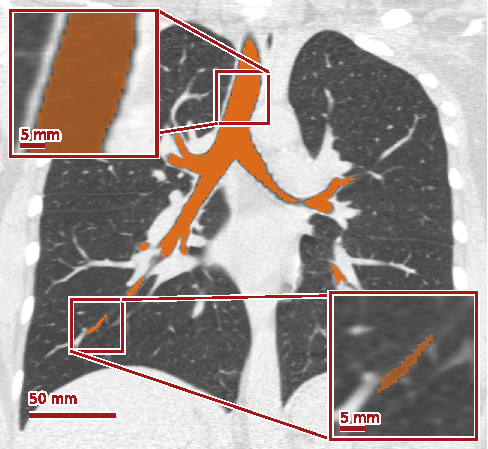
\includegraphics[width=\linewidth]{Figures/pdf/intro/airway_overview_slice.pdf}
    \caption{Coronal slice, reference airway overlaid. Both insets span
    \airwayInsetBox{}~mm; the magnified airways measure \airwayTracheaDiameter{}~mm
    and \airwayDistalDiameter{}~mm across.}
    % depth variant: Coronal slice, reference airway overlaid and split at branch
    % depth~\airwayProximalMaxGen{}. Both insets span \airwayInsetBox{}~mm; the
    % magnified airways measure \airwayTracheaDiameter{}~mm and
    % \airwayDistalDiameter{}~mm across.
    \label{fig:airway-overview-slice}
  \end{subfigure}\hfill
  \begin{subfigure}[b]{0.39\textwidth}
    \centering
    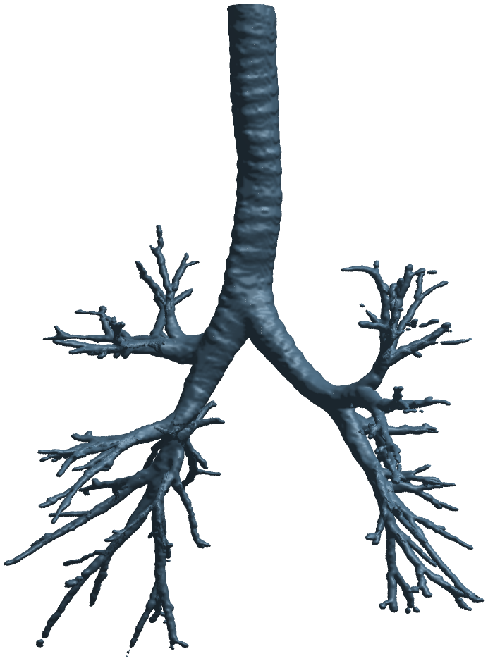
\includegraphics[width=\linewidth]{Figures/pdf/intro/airway_overview_tree_plain.pdf}
    \caption{The same tree in three dimensions.}
    % depth variant: The same tree, coloured by branch depth.
    \label{fig:airway-overview-tree}
  \end{subfigure}
  \caption[The airway tree in thoracic CT]{The airway tree in thoracic CT. ATM'22 case
  001~\cite{zhang2023atm22}, rendered for this study.}
  \label{fig:airway-overview}
\end{figure}

\section{Challenges in airway segmentation}
\label{sec:challenges}

Airway segmentation is difficult because two forms of imbalance occur simultaneously. The
first is the imbalance between airway foreground and background. Within the lung region supplied to the
network, annotated airway voxels form only a small fraction of the total volume
(Figure~\ref{fig:class-imbalance}). Moreover,
airway lumen and surrounding lung parenchyma can occupy overlapping intensity ranges, meaning
that the airway cannot be identified from voxel intensity alone. This becomes increasingly
important in peripheral branches, where the airway diameter approaches the spatial resolution
of the CT image and partial-volume effects reduce the distinction between lumen, airway wall
and surrounding tissue~\cite{montaudon2007,GarciaUceda2021AirwayCNN}.

A second imbalance exists within the airway foreground itself. The trachea and proximal
bronchi contain substantially more voxels than the numerous narrow distal branches. Consequently, the smallest
peripheral branches account for a small share of the segmented volume despite disproportionately determining the anatomical
extent of the reconstructed tree. A voxel-overlap objective such as Dice~\cite{dice1945association} is therefore dominated by the larger proximal structures
and can remain favourable even when a considerable proportion of the peripheral tree is absent~\cite{zhang2023atm22,zheng2021gradient}. 
This distinction is particularly important because airway segmentation is not simply a problem of recovering
foreground voxels, but of recovering a connected branching structure. A small discontinuity near a bifurcation may disconnect an
otherwise correctly segmented distal subtree while producing only a minor change in global
overlap.

% Placed after the two imbalance paragraphs because it evidences both: the rarity and
% intensity overlap of paragraph one, and the proximal/distal split of paragraph two.
% First referenced in paragraph one, so [tbp] can put it at the top of that page.
%
% The caption now defines generation depth and the proximal/distal split, so the
% panel legend is self-contained. What it deliberately does NOT carry is the
% justification for drawing the line there rather than at the clinical small-airway
% definition (under 2 mm, near generation eight), which sits below CT resolution and
% is largely absent from the annotation. That argument is prose, not caption; it is
% still only in the superseded section and should move up if it is wanted at all.
%
% The whole-scan version of this figure (denominator = uncropped volume, y-axis clipped above
% the parenchyma mode with the field-of-view air spike annotated) is still produced by
% dissertation/scripts/generate_hu_imbalance_histogram.py as
% Figures/pdf/background/airway_class_imbalance.pdf. It was cut deliberately: its extra
% content is the motivation for lung cropping, and its severity is partly produced by voxels
% preprocessing discards. Re-include it only if that motivation needs a figure of its own.
\begin{figure}[htbp]
  \centering
  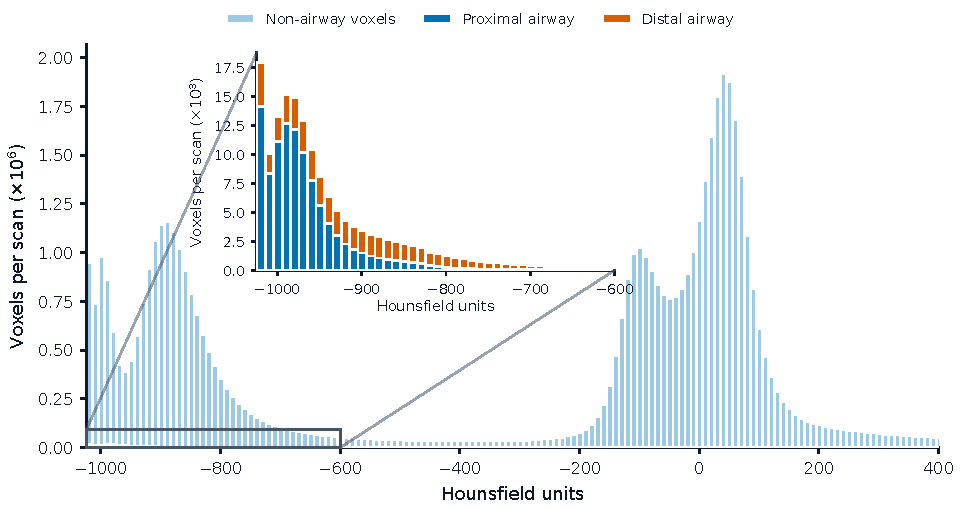
\includegraphics[width=\textwidth]{Figures/pdf/background/airway_class_imbalance_roi.pdf}
  \caption[Airway class imbalance by generation depth]{Hounsfield distribution of the lung
  region the network is trained on, over the \airwayNcases{} ATM'22 training scans. The airway
  window is magnified in both axes and split by generation depth: generation counts branch
  depth from the trachea (generation zero), so proximal is depth \airwayProximalMaxGen{} or
  less (trachea, main and lobar bronchi) and distal is everything beyond.}
  \label{fig:class-imbalance}
\end{figure}

Consequently, Dice overlap alone does not fully describe airway-tree quality. Airway benchmarks such as
ATM'22~\cite{zhang2023atm22} therefore complement volumetric overlap with measures such as tree-length-detection (TLD) and
branch-detection (BD). These measures emphasise recovery of the reference tree, 
but must themselves be interpreted alongside precision since overprediction may increase apparent tree coverage.

The same properties that make peripheral airways difficult to segment also make them difficult
to annotate. Dense three-dimensional airway masks are slow and expert-intensive to produce;
the reference annotations used by ATM'22 required approximately 60--90 minutes per scan~\cite{zhang2023atm22}. 
Annotation also becomes increasingly uncertain towards the distal tree,
where branches become narrow and poorly resolved. As a result, large collections of CT can be available
without their corresponding complete airway annotation. This motivates semi-supervised learning:
rather than requiring every training volume to carry a dense reference mask, unlabelled CT can potentially
provide an additional training signal by introducing wider anatomical variation.

\section{Prior work and unresolved gap}

Modern airway segmentation methods are predominantly based on encoder--decoder convolutional
networks derived from U-Net. In particular, nnU-Net provides a strong baseline because it
configures preprocessing, image spacing, patch size, network architecture, augmentation,
training schedule and inference around the properties of the dataset rather than treating the
network architecture in isolation~\cite{isensee2021nnunet}. This is important when evaluating additional
losses or training strategies: comparing different pipelines changes several factors
simultaneously, whereas a matched intervention within the same pipeline allows the effect of a
single component to be isolated.

Airway-specific methods have attempted to improve peripheral recovery through class weighting,
small-airway oversampling, skeleton-based hard-example mining and explicit reconnection of
broken branches~\cite{qin2019airwaynet,yu2022break,zhang2023atm22}. Results from ATM'22 suggest
that improvements in tree completeness arise from the complete training pipeline rather than
from a single loss function. The challenge results also illustrate an important limitation of
pure volumetric optimisation: methods with similar overlap can differ substantially in detected
tree length and branch recovery~\cite{zhang2023atm22}. This motivates incorporating geometry
directly when comparing airway predictions.

One such representation is clDice, which measures agreement using the centreline support of
two tubular masks~\cite{shit2021cldice}. Unlike volumetric Dice, its directional terms distinguish
between missing reference structure and additional predicted structure. It therefore provides
a natural geometry for measuring consistency between two airway predictions. However, clDice
does not itself guarantee anatomical correctness: the published topological result concerns
binary masks, whereas training requires finite differentiable skeletonisation of probability
maps. It is also relatively insensitive to airway calibre, and branches contribute according to
their length. For this reason, clDice is not
treated here as a replacement for conventional supervised objectives or evaluation metrics.
Instead, it is used as the geometry in which consistency between student and teacher
predictions is encouraged.

Semi-supervised segmentation methods attempt to exploit unlabelled images in addition to a
smaller labelled set. Pseudo-labelling assigns discrete labels to unlabelled examples before
using them as additional training targets. Mean Teacher instead maintains a second network
whose parameters are an exponential moving average of the student parameters and encourages
the student's prediction to remain consistent with the teacher under perturbation~\cite{tarvainen2017mean}. Importantly, the original Mean Teacher formulation supplies a
continuous teacher prediction rather than a thresholded pseudo-label.

Conventional Mean Teacher formulations enforce consistency voxel by voxel. Because background
voxels greatly outnumber airway voxels, accumulated background disagreement can dominate a
voxelwise objective even under patch-based training~\cite{zheng2021gradient}. The errors that matter clinically are also of the wrong kind for
such an objective: losing a narrow peripheral branch changes only a small number of foreground voxels
while removing a segment of the tree. This motivates asking whether consistency defined on
airway centreline geometry supplies a more useful unlabelled training signal than voxelwise
agreement alone, and that question is answered here by training both.

This distinction may matter particularly for airway segmentation. A label-starved teacher may
assign weak but non-zero probability to a peripheral branch that it does not recover at the
final inference threshold. Thresholding that prediction before computing consistency removes
this information entirely and makes the target behave more like online pseudo-labelling.
Conversely, retaining the continuous probability map preserves uncertainty, but does not
guarantee that the student will discover anatomy absent from the teacher. The central question
is therefore whether teacher-derived consistency can add peripheral structure or whether it
primarily consolidates the structures already represented by the teacher.

Existing semi-supervised work provides limited evidence for this question in sparse tubular
segmentation. An influential three-dimensional Mean Teacher application studied the
comparatively dense left atrium rather than a branching tree~\cite{yu2019uamt}.
Airway- and vessel-specific studies instead use feature specialisation, cross-geometry and
distance consistency, or pseudo-labelling to accommodate thin structures
~\cite{gu2023featurespecialisation,zhu2024crossgeometry,zhao2025vesselselftraining}. These studies
support the premise that voxel agreement alone may be insufficient, but their labelled fractions,
data and comparison pipelines differ. Semi-supervised models may also receive additional
optimisation, augmentation exposure or EMA inference relative to their supervised baselines.
Without a continuation control sharing that training envelope, an observed difference cannot be
assigned uniquely to the unlabelled consistency objective.

The unresolved gap addressed in this dissertation is therefore not simply whether a
semi-supervised model can obtain a higher headline Dice score. It is whether a
geometry-aware Mean Teacher can exploit unlabelled thoracic CT to recover airway-tree
structure beyond that learned from a limited labelled set, under the closest available matched
training comparison. A second question is whether any change is localised by airway calibre and
branch depth, and whether it is specific to centreline-aware rather than voxelwise agreement.

\section{Aim and objectives}

The aim of this dissertation is to determine whether geometry-aware Mean Teacher consistency
on unlabelled thoracic CT can improve airway-tree recovery under limited labelled supervision,
and to identify the mechanism by which any improvement or failure occurs.

To address this aim, the study:

\begin{enumerate}
    \item reports a label-limited supervised seed and a more fully labelled supervised model as
    scale references for the semi-supervised configurations;

    \item implements a two-stream Mean Teacher framework in which student predictions on
    unlabelled CT are regularised against an exponential-moving-average teacher using
    centreline-aware consistency;

    \item compares this model with a no-consistency continuation using the same training
    configuration;

    \ifshowcurrentcontrol
    \begin{currentcontrolroute}
    The available checkpoints estimate a configuration contrast but do not isolate consistency
    from independently realised output heads and training trajectories.
    \end{currentcontrolroute}
    \fi

    \ifshowpairedcontrol
    \begin{pairedcontrolroute}
    Prospective seed pairs additionally share the complete initial state and stochastic schedule,
    allowing variation in the fold-0 treatment effect to be estimated.
    \end{pairedcontrolroute}
    \fi

    \item tests consistency objective and weight as ablations, while
    separating changes in unlabelled pool size from changes in its training exposure;

    \item evaluates the resulting models using complementary volumetric and topology-aware
    measures, including Dice, detected tree length, branch detection and topology
    precision; and

    \item evaluates the final ordering on a held-out test cohort and on the external AeroPath
    dataset without dataset-specific tuning~\cite{stoverud2023aeropath}.
\end{enumerate}

The following chapter describes the datasets, nnU-Net training pipeline, Mean Teacher
implementation and matched experimental controls. The subsequent chapters report the
experimental results, interpret the observed behaviour and consider the implications and
limitations of geometry-aware semi-supervised learning for airway segmentation.
